\tikzset{
	A/.pic={
        code={
\draw[black](0,0)node[rotate=00]{\small \texttt{Built-dir}};
\draw[black](0,-0.5)node[rotate=00]{\small \texttt{Executable}};
\draw[black](0,-0.9)node[rotate=00]{\small \texttt{o-files}};
\draw[black](0,-1.3)node[rotate=00]{\small \texttt{...}};
\draw[black](0,-1.7)node[rotate=00]{\small \texttt{Makefile}};
%\draw[black,thick](-0.5,-0.15)rectangle(0.5,0.15);   
							}
	}
}

\tikzset{
	B/.pic={
        code={
\draw[black](0,0)node[rotate=00]{\small \texttt{Src-dir}};
\draw[black](0,-0.5)node[rotate=00]{\small \texttt{.cpp-files}};
\draw[black](0,-0.9)node[rotate=00]{\small \texttt{.hpp-files}};
\draw[black](0,-1.3)node[rotate=00]{\small \texttt{...}};
\draw[black](0,-1.7)node[rotate=00]{\small \texttt{MakeLists.txt}};
							}
	}
}

\tikzset{
	C/.pic={
        code={
\draw[black](0,0)node[rotate=00]{\small \texttt{Headers}};
\draw[black](0,-0.5)node[rotate=00]{\small \texttt{Additional}};
\draw[black](0,-0.9)node[rotate=00]{\small \texttt{.hpp-files}};
\draw[black](0,-1.3)node[rotate=00]{\small \texttt{...}};
%\draw[black](0,-1.7)node[rotate=00]{\small \texttt{...}};
							}
	}
}



\tikzset{
	main/.pic={
        code={
%\draw[black](0,0.25)node[rotate=00]{\tiny \texttt{Project-dir}};
\draw[black](0,0)node[rotate=00]{\small \texttt{Example-dir}};
%\draw[black](0,0)node[rotate=00]{\small \texttt{MakeLists.txt}};
%\draw[black,thick](-0.5,-0.15)rectangle(0.5,0.15);   
							}
	}
}

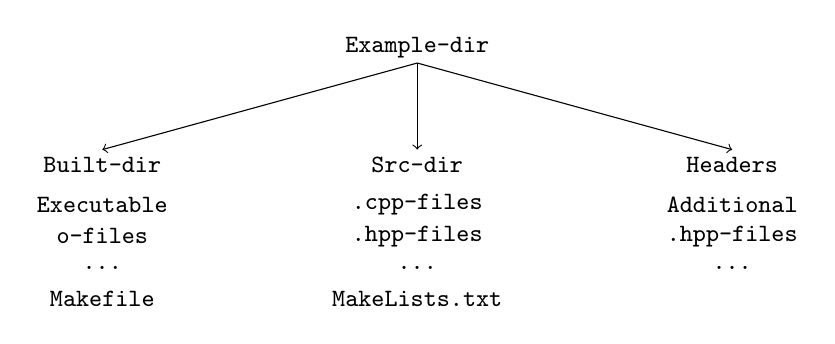
\begin{tikzpicture}
%Gitter
%\draw[step=0.5cm,very thin,black!20] (-6,-6) grid(6,6);
%\draw(-6,0)--(6,0);
%\draw(0,6)--(0,-6);

\path (0,3.5) pic {main};
\path (-4,2) pic {A};
\path (0,2) pic {B};
\path (4,2) pic {C};

\draw [black,->] (0,3.3)--(-4,2.2);
\draw [black,->] (0,3.3)--(0,2.2);
\draw [black,->] (0,3.3)--(4,2.2);
\end{tikzpicture}

